\documentclass{article}
\usepackage[utf8]{inputenc}
\usepackage{physics}
\usepackage{listings}
\usepackage{graphicx}
\usepackage{flexisym}

\title{Applied Mathematics TW324 Assignment 03}
\author{Bhekimpilo Ndhlela (18998712)}

\date{22 March 2018}

\begin{document}

\maketitle
\section*{Question 1}
\subsection*{a.)}
\subsection*{Python Source Code: }
\begin{lstlisting}[language=Python]
#!/usr/bin/python
def question_a(debug=True):
    global J
    J = [bessel_function(i) for i in xrange(0, 4)]

    if debug is True:
        print "\nDebug Mode : ON  \t Question 1 (a.)"
        print "i", "\t", "Jv(1)"
        for i in xrange(0, len(J)):
            print i, "\t", "{:.10f}".format(J[i])

def bessel_function(v, x=1, j=0):
    b = lambda k : pow(-1, k) * pow(float(x)/2, v + (2 * k)) \
                   / (sm.factorial(k) * sm.factorial(v + k))
    for k in xrange(0, 4):
        j = j + b(k)
    return j
\end{lstlisting}


\begin{center}
    \begin{tabular}{||c |c c c c||} 
    \hline
    $v$ & 0.0 & 1.0 & 2.0 & 3.0 \\ [0.5ex] 
    \hline\hline
    J_v(1) &  0.7651909722 & 0.4400499132 & 0.1149034288 & 0.0195633500  \\ [1ex] 
    \hline\hline 
    \end{tabular}
\end{center}
\pagebreak


\subsection*{b.)}
\subsection*{Python Source Code: }
\begin{lstlisting}[language=Python]
def question_b(debug=True):
    x = linspace(0,3, num=100)   # equally spaced points on interval [0, 3]
    x = [a for a in x if a != 0. if a != 1. if a != 2. if a != 3.]
    # the interpolating function from Barycentric Interpolation
    num = lambda v : (J[0]/v)-((3*J[1])/(v-1.))+((3*J[2])/(v-2.))-\
                     (J[3]/(v-3.))
    den = lambda v : (1./v)-(3./(v-1.))+(3./(v-2.))-(1./(v-3.))
    P = [num(i) / den(i) for i in x]
    global J
    J = [bessel_function(i) for i in x]

    # plot p(v) and Jv(1) on the same system
    func1, = plt.plot(x, J, label="Jv(1)", linestyle='--')
    func2, = plt.plot(x, P, label="P(v)", linestyle='-')
    plt.title('Jv(1) and P(v)')
    plt.ylabel('Jv(1) and P(v)')
    plt.xlabel('v')
    first_legend = plt.legend(handles=[func1], loc=1)
    ax = plt.gca().add_artist(first_legend)
    plt.legend(handles=[func2], loc=4)
    plt.show()
    # plot the error function Jv(1) - p(v)
    error = [jv - pv for jv, pv in zip(J, P)]
    plt.plot(x, error, 'r-')
    plt.title('Error Functioin')
    plt.ylabel('Error: Jv(1) - P(v)')
    plt.xlabel('v')
    plt.show()

    if debug is False:
        print "\nDebug Mode : ON  \t Question 1 (b.)"
        print "i \t\t x \t\t P(x) \t\t Jx(1) \t\t err"
        for i in xrange(len(x)):
            print i, "\t", "{:.10f}".format(x[i]), "\t", \
                           "{:.10f}".format(P[i]), "\t", \
                           "{:.10f}".format(J[i]), "\t", \
                           "{:.10f}".format(error[i])
    return error
\end{lstlisting}
\pagebreak

\begin{figure}[h!]
  \centering
  \begin{subfigure}{\linewidth}
    \includegraphics[width=\linewidth]{jv1_and_p.png}
    \caption{These are the J_v(1) and P(v) curves/ graphs }
  \end{subfigure}
  \begin{subfigure}{\linewidth}
    \includegraphics[width=\linewidth]{error.png}
    \caption{This is the error function: J_v(1) - P(v)}
  \end{subfigure}
\end{figure}

\pagebreak



\subsection*{c.)}
\subsection*{Python Source Code: }
\begin{lstlisting}[language=Python]
def question_c(error, M4=3.0, h=1.0, n=4.0, debug=True):
    est_error = (1. / (4. * n)) * (h**n) * M4
    max_error = sorted(error)[-1] # get max error from questio 1 b.)
    #compare errors is est_error >= max_error
    is_bound_true = est_error >= max_error

    if debug is True:
        print "\nDebug Mode : ON \t Question 1 (c.)"
        print "Estimated Error                \t:", est_error
        print "Maximum Error [Question 1 c.)] \t:", max_error
        print "est_error >= max_error ?       \t", is_bound_true
\end{lstlisting}

\begin{center}
    \begin{tabular}{||c| c||} 
    \hline
    \textbf{Estimated Error} & \textbf{Maximum Error [Question 1 b.)]} \\ [0.5ex] 
    \hline\hline
    0.18750000000000 & 0.0600749992108 \\ [1ex] 
    \hline
    \end{tabular}
\end{center}
\\
\\
\textbf{Theoretic Estimated Max Error $\geq$ Max Error [Question 1 b.)] ? \\
By taking $h = 1.0 $, I proved that: \\
 $C_n h^n M_n$ $\geq$ $max_{x_1 \leq x \leq x_4} |f(x) - P_{n - 1}(x)|$  }
\pagebreak

\subsection*{d.)}
\subsection*{Python Source Code:}
\begin{lstlisting}[language=Python]
def question_d(debug=True):
    # coeff of : pi'(x) = 2x^3 -9x^2 + 11x - 3 = 0
    coeff = [2, -9, 11, -3]
    zeros = roots(coeff)

    pi_x = lambda x : x**4 - 6*(x**3) + 11*(x**2) - 6*x
    maxi = [pi_x(x) for x in zeros]
    if debug is True:
        print "\nDebug Mode : ON  \t Question 1 (d.)"
        for i, (zero, max_min) in enumerate(zip(zeros, maxi)):
            print i,'\t', "{:.10f}".format(zero), '\t', \
                          "{:.10f}".format(max_min),'\t',\
                          "{:.10f}".format(fabs(max_min))
\end{lstlisting}
\textbf{  \\  }
\textbf{$\pi(x) = x(x - 1)(x - 2)(x - 3)$\\
$\pi(x) = x^4 - 6x^3 + 11x^2 - 6x $\\
$\pi^' (x) = 4x^3 - 18x^2 + 22x - 6 $\\
let: $\pi^' (x) = 0$ \\
$ 0 = 4x^3 - 18x^2 + 22x - 6$\\
Therefore:\\
$x_1, \quad x_2, \quad x_3 = 2.6180339887,\quad 1.5000000000,\quad 0.3819660113 \quad respectively$ \\
Hence: \\
$\pi(x_1) = \pi(2.6180339887) = -1.0000000000  \quad\quad|\pi(2.6180339887)| = 1.0000000000$\\
$\pi(x_2) = \pi(1.5000000000) = 0.56250000000 \quad\quad|\pi(1.5000000000)| = 0.5625000000$ \\
$\pi(x_3) = \pi(0.3819660113) = -1.0000000000  \quad\quad|\pi(0.3819660113)| = 1.0000000000$\\\\
$max(1.0000000000; 0.5625000000; 1.0000000000)$ = $1.0000000000$\\\\
Hence: $ max_{x_0 \leq x \leq x_3} |\pi(x)| = 1.0000$ 
}
\pagebreak



\section*{Question 3}
\subsection*{a.)}
\subsection*{Python Source Code for)}
\begin{lstlisting}[language=Python]
def question_a(N=4, debug=True):
    x = zeros(N)
    x = [cos(((2 * k - 1) * pi)/(2 * N)) for k in xrange(1, N + 1)]
    # defining the chebyshev Vandermonde matrix where V = 4x4 Matrix
    V = C.chebvander(x, N - 1).T
    if debug is True:
        print "DEBUG MODE: ON [Question 3 (a.)]:"
        print "vector x   = ", x
        print "\nchebyshev Vandermonde matrix where V:      \n", V
    return x, V
\end{lstlisting}


\textbf{ x = 
\begin{bmatrix} 0.9238795325112867 & 0.38268343236508984 & -0.3826834323650897 & -0.9238795325112867 \end{bmatrix}}\\ \\ \\

\textbf{ let: V $=$ Chebyshev Vandermonde Matrix \\ 
v = \begin{pmatrix} 
 1.0 &  1.0 & 1.0 & 1.0 \\
  0.92387953 & 0.38268343& -0.38268343 &-0.92387953\\
  0.70710678 &-0.70710678 &-0.70710678 & 0.70710678\\
  0.38268343 &-0.92387953 & 0.92387953 &-0.38268343\\
 \end{pmatrix}}
\pagebreak


\subsection*{b.)}
\subsection*{Python Source Code:}
\begin{lstlisting}[language=Python]
def question_b(x, V, debug=True):
    # finding the e^xi for the x elements
    exp_x = [exp(i) for i in x]
    V_inv = inv(V)
    c = matmul(V_inv, exp_x)
    if debug is True:
        print "\nDEBUG MODE: ON [Question 3 (b.)]:"
        print "vector e^x = ", exp_x
        print "\n(chebyshev Vandermonde matrix)^-I where V :\n", V_inv
        print "\nVc=exp(x)=> c=inv(V)exp(c) <=> inv(V)V=I  :\n", c
\end{lstlisting}

\[ \textbf{ e^x =  \begin{bmatrix} 2.5190441714069842& 1.4662138007571095& 0.682028773350537& 0.39697596864348 \end{bmatrix}} \]

\[Vc = e^x \]
\[V^{-1} Vc = V^{-1} e^x \]
\[c = V^{-1} e^x \]

\[
\textbf{c} = 
  \begin{pmatrix}  0.25 & 0.46193977 & 0.35355339 & 0.19134172\\
0.25 & 0.19134172 & -0.35355339 & -0.46193977\\
 0.25 & -0.19134172 & -0.35355339 & 0.46193977\\
 0.25 & -0.46193977 & 0.35355339 & -0.19134172 \end{pmatrix} 
  \begin{pmatrix} 2.5190441714069842\\ 1.4662138007571095\\ 0.682028773350537\\ 0.39697596864348 \end{pmatrix}
\]

\[ \textbf{c} = \begin{pmatrix} [ 1.62415515 & 0.48579634 & 0.29145858 & 0.1176341 \end{pmatrix} \\ \\ \]

\textbf{The vector c is the coeficient vector since: \\
Vc = y = exp(x) = $e^x$}

\pagebreak




\subsection*{c.)}
\subsection*{Python Source Code:}
\begin{lstlisting}[language=Python]
def question_c(b=3, a=0, N=0.0, debug=True):
    approx = lambda N : exp(N) * ((b-a)**N / (fact(N) * 2**(2*N-1)))
    while 10**-10 <= approx(N):
        N = N + 1.0
        print N
    if debug is True:
        print "\nDEBUG MODE: ON [Question 3 (c.)]:"
        print "Number of Chebyshev Points N = ", int(N)
        print "Approximated Value,      @ N = ", approx(N)
    return N
\end{lstlisting}

\textbf{The number of Chebyshev Points necessary to approximate the function exp(x) to an accuracy of 10 −10 on the interval $[0, 3]$ is :\\
\[n = 19\] \\ Approximated Value at,  $n = 19 $ is $ 1.24077928729e-11$}


\pagebreak

\subsection*{d.)}
\subsection*{Python Source Code:}
\begin{lstlisting}[language=Python]
def question_d(N, debug=True):
    chebyshev_points = zeros(int(N))
    chebyshev_points = [3./2. + 3./2.*cos(((2 * k - 1) * pi)/(2 * N)) \
                        for k in xrange(1, int(N) + 1)]
    if debug is True:
        print "\nDEBUG MODE : ON [Question 3 d.)]"
        print "The n Chebyshev Point where n = ", int(N)
        print "i", "\t", "Chebyshev_Points"
        for i, value in enumerate(chebyshev_points):
            print i, "\t", value
    return chebyshev_points
\end{lstlisting}

\begin{center}
    \begin{tabular}{||c| c||} 
    \hline
    \textbf{i } & \textbf{Chebyshev_Points} \\ [0.5ex] 
    \hline\hline
    1  &  2.99487673951\\[1ex] 
    \hline
    2  &  2.95410039891\\[1ex]
    \hline
    3  &  2.87365998998\\[1ex]
    \hline
    4  &  2.75574971739\\[1ex]
    \hline
    5  &  2.60358586601\\[1ex]
    \hline
    6  &  2.42131906903\\[1ex]
    \hline
    7  &  2.21392108956\\[1ex]
    \hline
    8  &  1.98704920381\\[1ex]
    \hline
    9  &  1.74689188542\\[1ex]
    \hline
    10 &  1.50000000000\\[1ex]
    \hline
    11 &   1.25310811458\\[1ex]
    \hline
    12 &   1.01295079619\\[1ex]
    \hline
    13 &   0.786078910444\\[1ex]
    \hline
    14 &     0.578680930965\\[1ex]
    \hline
    15 &   0.39641413399\\[1ex]
    \hline
    16 &  0.244250282606\\[1ex]
    \hline
    17 &  0.126340010017\\[1ex]
    \hline
    18 &   0.045899601091\\[1ex]
        \hline
    19 &    0.0051232604\\[1ex]
    \hline
    \end{tabular}
\end{center}


\pagebreak

\subsection*{e.)}
\subsection*{Python Source Code:}
\begin{lstlisting}[language=Python]
def question_e(chebyshev_points, debug=True):
    exp_xk = [exp(vk) for vk in chebyshev_points]
    #use polyfit
    fit = polyfit(chebyshev_points, exp_xk, len(exp_xk) - 1)
    err_vals = [e - f for e, f in zip(exp_xk, fit)]
    warnings.simplefilter('ignore', RankWarning) #ignore warnings
    # plot the error function
    plt.plot(linspace(0,3,num=19), exp_xk, label="exp(xk)")
    plt.plot(linspace(0,3,num=19), err_vals, label="err_vals")
    plt.plot(linspace(0,3,num=19), fit, label="fit")
    plt.legend(bbox_to_anchor=(1.0, 1), loc=0, borderaxespad=0.)
    plt.show()
    if debug is True:
        print "\nDEBUG MODE : ON  [Question 3 e.)]"
        print "k", "\t", "chebyshev_points(k)", "\t", "exp(k)\t\t\t",\
              "polyfit_points(k)"
        for k, (xk, e) in enumerate(zip(chebyshev_points, exp_xk)):
            print k, "\t", "{:.16f}".format(xk), "\t","{:.16f}".format(e), \
                  "\t", "{:.16f}".format(fit[k])
\end{lstlisting}

\begin{figure}[h!]
  \centering
  \begin{subfigure}{\linewidth}
    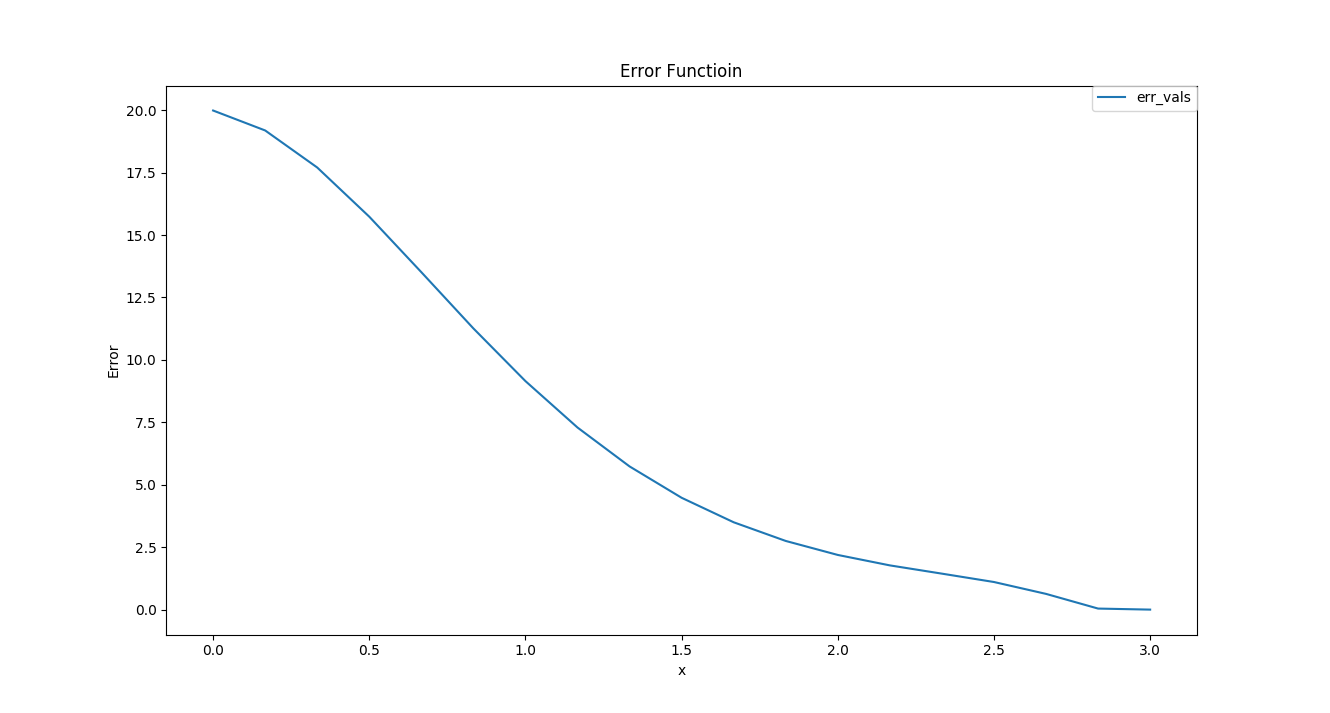
\includegraphics[width=\linewidth]{Figure_11.png}
    \caption{Error of \textbf{e^x} }
  \end{subfigure}
\end{figure}

\pagebreak


\begin{center}
    \begin{tabular}{||c| c |c| c||} 
    \hline
    \textbf{k } & \textbf{chebyshev_points(k)} & \textbf{exp(k)} & \textbf{polyfit_points(k)} \\ [0.5ex] 
    \hline\hline
1      & 2.9948767395100049  &    19.9828966364183991&     -0.0000000000000168 \\[1ex] 
\hline
2     &  2.9541003989089956   &   19.1844565966013114 &    0.0000000000004260 \\[1ex]
\hline
3    &   2.8736599899825861    &  17.7016877825937016  &   -0.0000000000047462 \\[1ex] 
\hline
4   &    2.7557497173937930     & 15.7328316599325380   &  0.0000000000335313 \\[1ex]
\hline
5  &     2.6035858660096975      &13.5121038604438937    & -0.0000000001397079 \\[1ex] 
\hline
6 &      2.4213190690345021&      11.2607031675513909     &0.0000000006593969 \\[1ex] 
\hline
7&       2.2139210895556101 &     9.1515301018746555&      0.0000000008709762 \\[1ex] 
\hline
8       &1.9870492038070253  &    7.2939789307318259 &     0.0000000272904685 \\[1ex] 
\hline
9      & 1.7468918854211006   &   5.7367444785709703  &    0.0000002724300402 \\[1ex] 
\hline
10    &   1.5000000000000000   &   4.4816890703380645  &    0.0000027591227060 \\[1ex] 
\hline
11   &   1.2531081145788994     & 3.5012082197865295    &  0.0000247987718511 \\[1ex] 
\hline
12  &    1.0129507961929751      &2.7537146890514030     & 0.0001984144914214 \\[1ex] 
\hline
13 &     0.7860789104443897&      2.1947736279721375      &0.0013888880233439 \\[1ex] 
\hline
14&      0.5786809309654983 &     1.7836840758813131&      0.0083333336421386 \\[1ex] 
\hline
15     & 0.3964141339903027  &    1.4864847939769930 &     0.0416666665889665 \\[1ex] 
\hline
16    &  0.2442502826062074   &   1.2766638172542299  &    0.1666666666793699 \\[1ex] 
\hline
17   &   0.1263400100174137    &  1.1346679011556191   &   0.4999999999988355 \\[1ex] 
\hline
18  &    0.0458996010910044     & 1.0469692911054875    &  1.0000000000000446 \\[1ex] 
\hline
19 &     0.0051232604899951      &1.0051364068301394     & 1.0000000000000009 \\[1ex] 
\hline
    
    \hline
    \end{tabular}
\end{center}
\textbf{}





\end{document}


